\documentclass[10pt,letterpaper]{article}
\usepackage[margin=0.9in]{geometry}
\usepackage[T1]{fontenc}
\usepackage{lmodern}
\usepackage{amsmath,amssymb,graphicx,booktabs,array,xcolor,float,caption,fancyhdr}
\usepackage[colorlinks=true,linkcolor=blue!45!black,urlcolor=blue!45!black]{hyperref}
\usepackage{url}
\hypersetup{pdftitle={Sparse Dominating Sets Revisited: Supplementary Technical Report},pdfauthor={},pdfsubject={Supplementary experimental evidence, lightweight artifact version 0.3}}
\graphicspath{{figures/}}
\renewcommand{\thesection}{\Alph{section}}
\renewcommand{\thetable}{S\arabic{table}}
\renewcommand{\thefigure}{S\arabic{figure}}
\captionsetup{font=small,labelfont=bf}
\setlength{\parskip}{2pt}
\setlength{\parindent}{1em}
\setlength{\headheight}{14pt}
\pagestyle{fancy}
\fancyhf{}
\lhead{\small Sparse Dominating Sets Revisited}
\rhead{\small Supplementary report v0.3}
\cfoot{\thepage}
\newcommand{\Ratio}{\textsf{Ratio}}
\newcommand{\Rplus}{\textsf{Ratio+}}
\newcommand{\Degree}{\textsf{Degree}}
\newcommand{\Random}{\textsf{Random-Prune}}
\newcommand{\CC}{CC$^2$FS}
\newcommand{\tablefont}{\fontsize{9}{11}\selectfont}
\newcommand{\smalltablefont}{\fontsize{8.5}{10.5}\selectfont}
\newcommand{\sourceid}[1]{\nolinkurl{#1}}
\begin{document}
\thispagestyle{plain}
\begin{center}
{\Large\bfseries Sparse Dominating Sets Revisited:\\[3pt]
Supplementary Technical Report}\par
\vspace{7pt}
{\small Companion to \emph{Sparse Dominating Sets Revisited: Logarithmic Approximation and Tight Congestion Bounds}}\par
\vspace{6pt}
{\small Lightweight artifact v0.3 \quad 9 November 2026}
\end{center}

\section*{Scope and reading guide}
This report provides additional evidence and experimental detail for the companion manuscript. It develops three aspects of the evaluation: the costs of computing the same greedy landmark sequence, the behavior of landmark partitions under controlled resources, and the complete latency of exact neighborhood-subgraph extraction. The principal theorems and their complete proofs appear in Sections IV--VI of the companion manuscript.

The report follows the manuscript's graph cohorts. Implementation measurements use its five large SNAP networks and uk-2002; retrieval measurements use Stanford, Google, in-2004 and eu-2005. The four retrieval graphs are evaluated with the competing selectors, random seeds, query strata and BFS controls described in the following sections.

\begin{table}[H]
\centering\small
\caption{Relationship to the companion manuscript.}
\begin{tabular}{@{}p{.06\linewidth}p{.32\linewidth}p{.54\linewidth}@{}}
\toprule
Part & Manuscript topic & Additional material in this report\\
\midrule
A & Efficient implementation & Phase costs and all twelve conditions in the completed multi-radius rerun cohort.\\
B & Candidate selectivity & Budget utilization, fixed-count index and partition statistics, and query-stratum comparisons.\\
C & Neighborhood retrieval & Complete extraction results, uncertainty, secondary queries and BFS controls for four graphs.\\
D & Robustness & Full final-tie sensitivity table for the five main SNAP graphs.\\
E & Experimental setup & Measurement contracts, evidence provenance and display-reproduction instructions.\\
\bottomrule
\end{tabular}
\end{table}

\paragraph{Notation and methods.}
Let $G=(V,E)$ be a simple undirected graph. A landmark set $D$ covers every vertex within landmark radius $r$, and its average congestion is
\[
\kappa_r(D)=\frac{1}{|V|}\sum_{u\in D}|N_r[u]|.
\]
\Ratio\ selects the vertex maximizing newly covered vertices divided by neighborhood size; \Degree\ maximizes the newly covered count. \Rplus\ breaks equal ratios by larger newly covered counts, while Degree+ uses the ratio as its secondary priority. Final ties use vertex IDs unless the experiment explicitly varies this order. \Random\ deletes landmarks while preserving coverage, and \CC\ is the weighted local-search baseline described in the manuscript. Query radius $h$ and query seed-set size $|Q|$ are distinct from the landmark radius $r$.

\paragraph{Two retrieval experiments.}
Section~\ref{sec:structure} uses the existing candidate-selectivity cohort, with 6,800 queries per graph. Section~\ref{sec:query} uses fresh queries and returns an exact induced subgraph, including sorted vertex and undirected-edge buffers. Candidate retrieval and exact-subgraph extraction are measured as separate tasks. The two completed exact-subgraph batches contain 8,000 primary queries and 3,200 secondary queries across four graphs, with three timing repetitions per configuration. The source audits cover 1,276,800 timed query records in total.

\clearpage
\section{Implementation costs and larger radii}
\label{sec:implementation}
\subsection{Where the implementation saves time}
The counter-and-heap implementation changes how greedy scores are maintained. Once a vertex becomes covered, its contribution is removed from the affected counters; the algorithm need not recompute complete neighborhood intersections after each selection. Under the same primary, secondary and final tie priorities, the new implementation produces the same complete landmark sequence as the reference. Consequently, the implementation comparison isolates computation and storage costs rather than a change in solution quality.

Figure~\ref{fig:phases} decomposes the $r=1$ Ratio runs into input, neighborhood/data-structure preparation, selection and output. The five SNAP graphs use five repetitions per implementation; uk-2002 uses three. Every phase is summarized by its own median. The whole-process measurement is an external start-to-exit time and additionally includes startup, shutdown and other overhead. Independent phase medians therefore need not sum to the median whole-process time.

\begin{figure}[H]
\centering
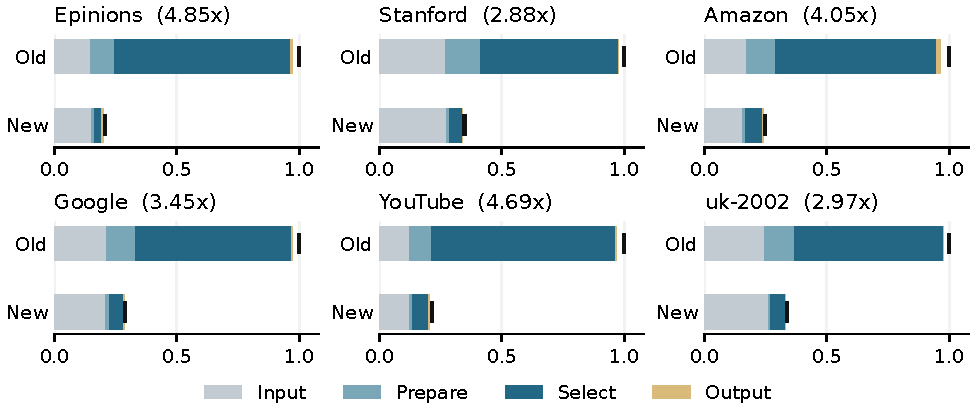
\includegraphics[width=\linewidth]{implementation_phases.pdf}
\caption{Ratio phase costs at $r=1$, divided by the reference implementation's median whole-process time on each graph. Black ticks mark whole-process times; panel labels give whole-process speedups. Stacked segments are independently computed phase medians.}
\label{fig:phases}
\end{figure}

\paragraph{Selection and preparation.}
The selection phase improves by approximately $9.7$--$22.9\times$ on the five SNAP graphs; on uk-2002 it improves by $10.3\times$. Neighborhood/data-structure preparation also decreases. These savings explain why the implementation advantage remains substantial even though the choice of landmarks is unchanged. The report's machine-readable phase table retains all absolute measurements, including input and output, rather than only the normalized figure.

\paragraph{The input floor.}
Input costs change little compared with selection costs. For example, uk-2002 input takes $67.75$ seconds in the reference and $72.12$ seconds in the new implementation, while selection falls from $168.27$ to $16.40$ seconds. Input alone accounts for approximately $77\%$ of the new whole-process time. Thus a larger selection-stage speedup does not imply an equally large end-to-end speedup. The whole-process speedup is $2.97\times$ on this graph, including its input cost.

\paragraph{Measurement controls.}
Both implementations use the same graph, vertex order, greedy strategy and compiler flags on the same pinned core. Coverage, objective value and ordered landmark output are independently checked. This phase comparison uses 50 Ratio records on the five SNAP graphs and six on uk-2002, a subset of the manuscript's four-strategy validation collection.

\clearpage
\subsection{Complete multi-radius rerun cohort}
At larger radii, explicitly represented neighborhoods become much larger. Table~\ref{tab:radius} reports every condition in the completed Stanford reference-implementation rerun cohort: the full graph and five sampled views, each at $r=2,3$. The 50,000-vertex views use seeds 20261105 and 20261107; the 100,000-vertex views use these seeds and 20261106. The table lists each size, seed and radius combination in the cohort.

\begin{table}[H]
\centering\smalltablefont\setlength{\tabcolsep}{4pt}
\caption{All twelve multi-radius conditions. Entries are three-run medians. View seed suffixes 05/06/07 denote 20261105/06/07. Speedup is old/new whole-process time; saved memory is $100(1-\mathrm{new}/\mathrm{old})$.}
\label{tab:radius}
\begin{tabular}{@{}lrrrrrrr@{}}
\toprule
View / seed & $r$ & Old (s) & New (s) & Speedup & Old GiB & New GiB & Saved (\%) \\
\midrule
50k / 05 & 2 & 886.9 & 40.6 & 21.82 & 63.57 & 5.77 & 90.9 \\
50k / 05 & 3 & 1458.6 & 106.2 & 13.74 & 101.75 & 8.31 & 91.8 \\
50k / 07 & 2 & 969.7 & 50.9 & 19.04 & 68.08 & 6.13 & 91.0 \\
50k / 07 & 3 & 1600.0 & 202.1 & 7.92 & 109.82 & 8.99 & 91.8 \\
100k / 05 & 2 & 1567.1 & 41.6 & 37.64 & 74.19 & 6.59 & 91.1 \\
100k / 05 & 3 & 4718.7 & 179.6 & 26.27 & 204.33 & 17.80 & 91.3 \\
100k / 06 & 2 & 1947.0 & 59.2 & 32.87 & 95.95 & 8.53 & 91.1 \\
100k / 06 & 3 & 3386.8 & 159.2 & 21.27 & 171.08 & 14.39 & 91.6 \\
100k / 07 & 2 & 1547.1 & 41.8 & 36.99 & 73.54 & 6.54 & 91.1 \\
100k / 07 & 3 & 4628.0 & 185.6 & 24.94 & 205.78 & 17.88 & 91.3 \\
Full graph & 2 & 2243.2 & 62.5 & 35.87 & 107.24 & 9.43 & 91.2 \\
Full graph & 3 & 6205.4 & 221.3 & 28.04 & 251.46 & 21.66 & 91.4 \\
\bottomrule
\end{tabular}

\end{table}

\paragraph{Observed scaling.}
The new implementation is faster in all twelve conditions, with speedups from $7.92$ to $37.64\times$. Peak RSS decreases by $90.9$--$91.8\%$. The full-graph endpoints highlighted in the manuscript belong to this wider set of paired observations. The table lists individual seeds to capture the neighborhood-density variation between sampled views.

\paragraph{Resource limits and timing.}
The reference implementation runs serially with a 320\,GiB address-space limit and unlimited wall/CPU time. The new implementation uses a 64\,GiB address-space limit. Table~\ref{tab:radius} reports the elapsed time and observed peak RSS of the completed runs.

Whole-process time covers native process startup, input, preprocessing, greedy selection, output and destruction. Independent validation time is excluded for both implementations. The runs use the same pinned server core. The separate pilot is excluded from the 36 formal reference runs.

\paragraph{Output agreement.}
The completion audit verifies all 36 formal reference runs, including independent coverage/cost checks and complete ordered-output agreement with the new implementation. Original source and binary identities are unchanged. These comparisons measure implementation efficiency at larger landmark radii.

\clearpage
\section{Resource controls and query-stratum selectivity}
\label{sec:structure}
\subsection{Budget matching and fixed-count index footprints}
All selectors use the same nearest-landmark partition and boundary-index code. Native landmarks are retained, and further landmarks follow a common augmentation order. Three caps are defined from the largest native index payload, with configurations chosen using bytes alone before query evaluation. Table~\ref{tab:budgets} audits the resulting 27 configurations per graph: four deterministic selectors and five random seeds at each of three caps. Graph adjacency is shared and excluded from these index-payload caps.

\begin{table}[H]
\centering\smalltablefont\setlength{\tabcolsep}{4pt}
\caption{Index caps and actual utilization across all matched-budget configurations. MiB means $2^{20}$ bytes. The query counts belong to the original candidate-selectivity cohort.}
\label{tab:budgets}
\begin{tabular}{@{}lrcrr@{}}
\toprule
Graph & Vertices & Caps (MiB), low/medium/high & Use (\%) & Queries \\
\midrule
Stanford & 255,265 & 7.78/8.95/10.11 & 95.39--100.00 & 6800 \\
Google & 855,802 & 27.82/31.99/36.17 & 95.90--100.00 & 6800 \\
in-2004 & 1,353,703 & 42.25/48.59/54.93 & 95.48--100.00 & 6800 \\
eu-2005 & 862,664 & 56.56/65.04/73.52 & 95.23--100.00 & 6800 \\
\bottomrule
\end{tabular}

\end{table}

The separate fixed-count control makes the number and mean size of pieces identical across selectors. Table~\ref{tab:structure} supplements the manuscript's candidate comparison with index and partition statistics. Random-P reports the mean of five independently constructed indexes; its candidate SD is the sample standard deviation of the five per-seed candidate means.

\begin{table}[H]
\centering\smalltablefont\setlength{\tabcolsep}{6pt}
\caption{Fixed-count index and partition statistics. Piece P99 and largest-piece size count vertices. For Random-P, each displayed statistic, including the maximum, is averaged over the five seed-specific values. Candidates are averaged over the 6,800 queries.}
\label{tab:structure}
\begin{tabular}{@{}lrrrrr@{}}
\toprule
Method & Index MiB & Piece P99 & Largest piece & Cand. ($10^3$) & Seed SD \\
\midrule
\multicolumn{6}{@{}l}{\textit{Stanford: 28,534 pieces; mean piece size 8.95}} \\
Ratio & 7.78 & 65.7 & 18,962 & 11.18 & -- \\
Ratio+ & 9.67 & 62.7 & 16,384 & 13.13 & -- \\
Degree & 10.26 & 65.0 & 13,990 & 11.84 & -- \\
CC$^2$FS & 9.95 & 60.0 & 14,902 & 13.66 & -- \\
Random-P & 9.96 & 65.3 & 12,568 & 12.12 & 0.36 \\
\midrule
\multicolumn{6}{@{}l}{\textit{Google: 212,524 pieces; mean piece size 4.03}} \\
Ratio & 27.82 & 31.0 & 1,584 & 1.73 & -- \\
Ratio+ & 29.19 & 27.0 & 3,344 & 2.19 & -- \\
Degree & 31.57 & 22.0 & 969 & 2.18 & -- \\
CC$^2$FS & 31.51 & 21.0 & 1,328 & 2.34 & -- \\
Random-P & 31.04 & 23.0 & 1,129 & 2.42 & 0.04 \\
\midrule
\multicolumn{6}{@{}l}{\textit{in-2004: 194,605 pieces; mean piece size 6.96}} \\
Ratio & 42.25 & 70.0 & 9,752 & 4.13 & -- \\
Ratio+ & 53.41 & 63.0 & 17,433 & 4.84 & -- \\
Degree & 62.99 & 59.0 & 11,481 & 4.18 & -- \\
CC$^2$FS & 62.90 & 57.0 & 12,580 & 4.29 & -- \\
Random-P & 60.17 & 60.8 & 11,165 & 4.21 & 0.09 \\
\midrule
\multicolumn{6}{@{}l}{\textit{eu-2005: 86,563 pieces; mean piece size 9.97}} \\
Ratio & 56.56 & 114.0 & 23,984 & 28.95 & -- \\
Ratio+ & 66.61 & 77.0 & 60,249 & 44.21 & -- \\
Degree & 75.53 & 75.0 & 13,975 & 34.90 & -- \\
CC$^2$FS & 75.27 & 63.4 & 25,138 & 37.84 & -- \\
Random-P & 74.53 & 71.8 & 16,896 & 35.17 & 0.66 \\
\bottomrule
\end{tabular}

\end{table}

\clearpage
\subsection{Interpreting the resource advantage}
At the common landmark count, Ratio uses less index space than each competing selector in Table~\ref{tab:structure} on all four graphs. It also returns fewer mean candidates than each competing selector, with Random-P interpreted as the five-seed mean. The candidate advantage is present at the same piece count and a smaller index footprint.

A query touches the union of pieces containing its answers, so candidate counts reflect both landmark placement and the resulting partition. Ratio's largest piece can exceed Degree's while its mean candidate count remains lower. The P99 and maximum piece sizes complement the query-level candidate measurements.

\subsection{All query strata at the lowest matched budget}
The original workload contains two start distributions: uniform starts (U) and degree-stratified starts (S). For each distribution, $h=1$ uses $|Q|=1,5,20$ with 1,000 queries per stratum; $h=2$ uses $|Q|=1,5$ with 200 queries per stratum. All selectors receive the same held-out queries and return candidates with complete recall.

\begin{figure}[H]
\centering
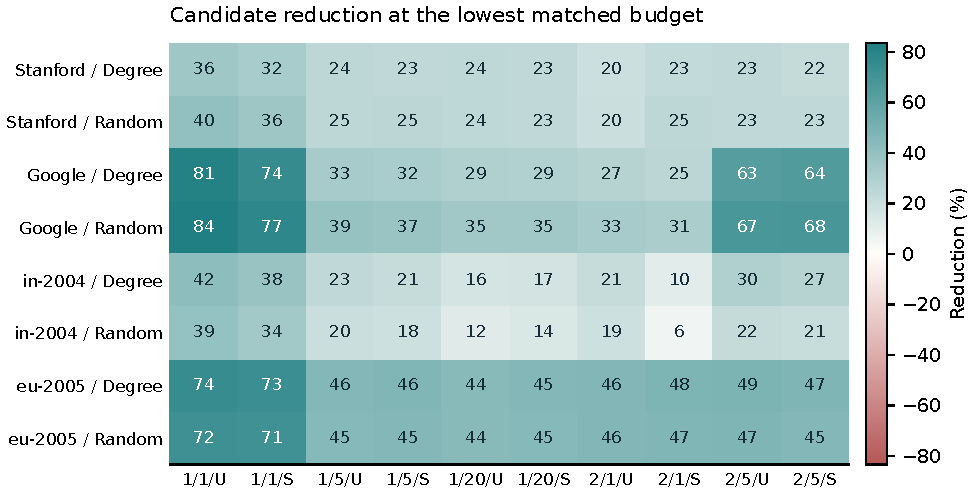
\includegraphics[width=\linewidth]{candidate_strata.pdf}
\caption{Candidate reduction, $100(1-C_{\mathrm{Ratio}}/C_{\mathrm{reference}})$, in every query stratum at the lowest matched index budget. Column labels are $h/|Q|/$start distribution. Random denotes the five-seed mean; positive values favor Ratio. Each cell uses the stratum mean, not an unweighted average of per-query ratios.}
\label{fig:candidate-strata}
\end{figure}

Ratio reduces mean candidates in all 80 graph--reference--stratum comparisons displayed in Figure~\ref{fig:candidate-strata}, by $5.5$--$83.5\%$. This is stronger evidence about consistency across query types than a single pooled mean: the lowest-budget advantage is present under both start distributions, both query radii and all tested query sizes. The range summarizes the stratum means displayed in the figure.

The candidate counts measure the amount of material admitted by the shared partition index. Whether this reduction lowers complete query time depends on subsequent reads, exact processing and output construction. Section~\ref{sec:query} measures those costs with a separate exact-subgraph task and fresh queries.

\clearpage
\section{Exact neighborhood-subgraph extraction}
\label{sec:query}
\subsection{Task, cohorts and measurement}
The new task returns the exact induced subgraph on the vertices within $h$ hops of an input seed set $Q$. Every method must produce the same sorted vertex and undirected-edge buffers. The partition path first uses the existing boundary index to obtain candidates and then performs the exact work needed to construct the output. Two BFS controls return the same output: one uses the original graph layout and the other uses each selector's physical layout. Original vertex IDs are preserved when layouts change.

The primary workload fixes $h=1$ and $|Q|=1$, with 1,000 uniform-start and 1,000 degree-stratified-start queries per graph. Each of the eight remaining strata has 100 queries and is reported separately as context. The Stanford/Google batch completed on 8 November 2026; the in-2004/eu-2005 extension completed on 9 November using the same engine and settings. Starts exclude the earlier development, test and pilot starts. Query sets and minimum-budget configurations were fixed before timing. A common $8n$-byte mapping is added to the original minimum-budget accounting for all selectors.

\begin{table}[H]
\centering\tablefont\setlength{\tabcolsep}{5pt}
\caption{Primary workload: all partition selectors. Times are in microseconds, requested bytes in KiB ($2^{10}$ bytes). Random-P averages five seed-specific means; its P95 entry is the mean of five seed-specific P95 values, not the percentile of a pooled distribution.}
\label{tab:query-methods}
\begin{tabular}{@{}llrrrr@{}}
\toprule
Graph & Method & Memory mean & Warm-file mean & Warm-file P95 & Req. KiB \\
\midrule
Stanford & Ratio & 70.82 & 284.10 & 1215.49 & 363.33 \\
 & Ratio+ & 111.62 & 757.92 & 3627.50 & 714.01 \\
 & Degree & 87.92 & 385.92 & 2172.91 & 402.09 \\
 & CC$^2$FS & 106.63 & 739.22 & 3222.32 & 631.91 \\
 & Random-P & 92.47 & 397.26 & 1890.66 & 439.97 \\
\midrule
Google & Ratio & 3.23 & 23.22 & 63.22 & 8.99 \\
 & Ratio+ & 4.54 & 27.05 & 80.16 & 13.11 \\
 & Degree & 6.50 & 32.31 & 92.04 & 14.62 \\
 & CC$^2$FS & 7.52 & 35.54 & 103.69 & 17.29 \\
 & Random-P & 7.08 & 34.48 & 100.74 & 16.13 \\
\midrule
in-2004 & Ratio & 33.74 & 127.29 & 750.41 & 252.91 \\
 & Ratio+ & 40.91 & 160.36 & 783.84 & 336.70 \\
 & Degree & 39.97 & 153.03 & 756.46 & 282.70 \\
 & CC$^2$FS & 40.80 & 169.05 & 766.24 & 305.86 \\
 & Random-P & 38.62 & 140.27 & 690.12 & 286.14 \\
\midrule
eu-2005 & Ratio & 103.27 & 319.18 & 1326.22 & 744.72 \\
 & Ratio+ & 197.99 & 1002.93 & 6254.17 & 1763.37 \\
 & Degree & 171.45 & 692.86 & 2500.83 & 1375.68 \\
 & CC$^2$FS & 223.67 & 1224.07 & 6066.19 & 1846.35 \\
 & Random-P & 165.75 & 702.78 & 2915.45 & 1314.28 \\
\bottomrule
\end{tabular}

\end{table}

Timing starts with the native query seeds and ends after complete sorted output buffers. It includes scratch reset, candidate/frontier reads, exact processing and output construction; independent correctness checks and warmup are excluded. Each configuration has three repetitions, collapsed to a median per query before aggregation. Table~\ref{tab:query-methods} gives means over those query-level values, while P95 describes their latency distribution. Memory and warm-file measurements are kept separate.

\clearpage
\subsection{Primary comparisons and BFS controls}
In the warm-file primary workload, Ratio reduces mean complete time by $16.8$--$53.9\%$ relative to Degree and $9.3$--$54.6\%$ relative to the Random-Prune mean across the four graphs. All eight corresponding 95\% time-ratio intervals lie below one (Table~\ref{tab:query-ci}). Requested adjacency bytes also decrease in all eight comparisons. The result supports the practical value of landmark choice within the shared partition-extraction pipeline.

\begin{table}[H]
\centering\tablefont\setlength{\tabcolsep}{5pt}
\caption{Primary warm-file comparisons. Ratios are Ratio/reference, so values below one favor Ratio. Confidence intervals are paired stratified bootstrap percentile intervals with 2,000 resamples; random configurations are resampled as well as queries.}
\label{tab:query-ci}
\begin{tabular}{@{}llrcrc@{}}
\toprule
Graph & Reference & Time ratio & 95\% CI & Byte ratio & 95\% CI \\
\midrule
Stanford & Degree & 0.736 & [0.692, 0.783] & 0.904 & [0.886, 0.921] \\
Stanford & Random-P & 0.715 & [0.671, 0.758] & 0.826 & [0.798, 0.852] \\
Google & Degree & 0.719 & [0.696, 0.742] & 0.615 & [0.596, 0.635] \\
Google & Random-P & 0.673 & [0.654, 0.694] & 0.557 & [0.539, 0.576] \\
in-2004 & Degree & 0.832 & [0.779, 0.887] & 0.895 & [0.821, 0.967] \\
in-2004 & Random-P & 0.907 & [0.859, 0.955] & 0.884 & [0.837, 0.932] \\
eu-2005 & Degree & 0.461 & [0.440, 0.483] & 0.541 & [0.524, 0.558] \\
eu-2005 & Random-P & 0.454 & [0.416, 0.506] & 0.567 & [0.517, 0.618] \\
\bottomrule
\end{tabular}

\end{table}

\paragraph{Uncertainty and aggregation.}
Uniform and degree-stratified queries receive equal weight in the primary aggregate. The bootstrap resamples queries within each stratum, keeping method observations paired. The random reference additionally resamples the five seed configurations. The intervals quantify sampling variation within the evaluated graph/workload configurations. Ratios divide the mean times of the compared methods. Separate workload-specific comparisons are retained in the frozen uncertainty files; all primary point estimates against Degree and Random-Prune are below one for both start distributions.

\begin{table}[H]
\centering\tablefont\setlength{\tabcolsep}{5pt}
\caption{Primary workload BFS controls. Times are mean microseconds. Same-layout BFS uses Ratio's physical layout. The last column divides Ratio partition time by same-layout BFS time.}
\label{tab:bfs}
\begin{tabular}{@{}llrrrr@{}}
\toprule
Graph & Mode & Ratio partition & Original BFS & Same-layout BFS & Ratio/same \\
\midrule
Stanford & Memory & 70.82 & 32.05 & 31.36 & 2.26 \\
Stanford & Warm file & 284.10 & 114.16 & 83.00 & 3.42 \\
Google & Memory & 3.23 & 2.34 & 2.33 & 1.38 \\
Google & Warm file & 23.22 & 42.95 & 29.57 & 0.79 \\
in-2004 & Memory & 33.74 & 23.47 & 23.44 & 1.44 \\
in-2004 & Warm file & 127.29 & 49.89 & 56.70 & 2.24 \\
eu-2005 & Memory & 103.27 & 78.46 & 78.62 & 1.31 \\
eu-2005 & Warm file & 319.18 & 158.05 & 178.64 & 1.79 \\
\bottomrule
\end{tabular}

\end{table}

Google's warm-file Ratio partition path is faster than both BFS controls. For Stanford, in-2004 and eu-2005, BFS remains faster; in memory, BFS is faster on all four graphs. The results compare landmark selection within the partition pipeline alongside direct traversal.

\clearpage
\subsection{Secondary workloads and cache scope}
Figure~\ref{fig:context} retains all eight secondary query strata on each graph. Each cell uses 100 newly generated queries. Warm-file mean time decreases in 24 of the 64 graph--reference--stratum comparisons. The figure reports each secondary stratum separately to show how performance varies with query size, radius and start distribution.

\begin{figure}[H]
\centering
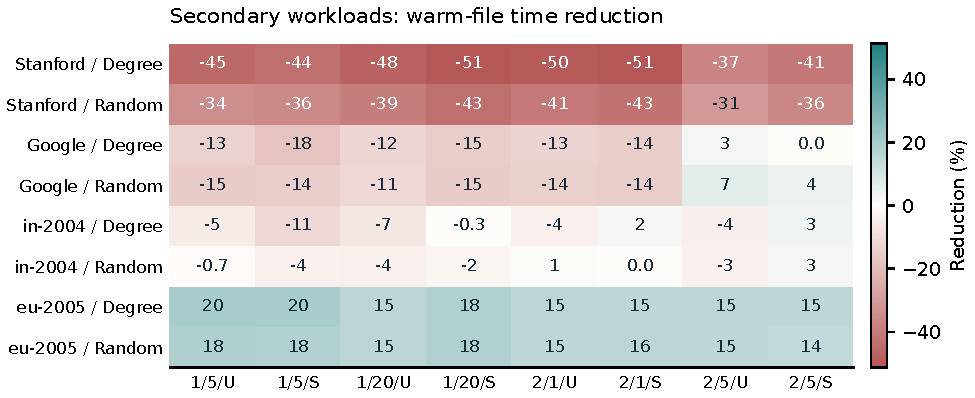
\includegraphics[width=\linewidth]{query_context.pdf}
\caption{Secondary strata: $100(1-T_{\mathrm{Ratio}}/T_{\mathrm{reference}})$ for complete warm-file query time. Labels are $h/|Q|/$start distribution, with U uniform and S degree-stratified. Positive values favor Ratio; negative values indicate additional time. Random denotes the five-seed mean.}
\label{fig:context}
\end{figure}

\paragraph{Reading volume and cache state.}
The shared reader deduplicates adjacency rows, coalesces contiguous reads and reuses rows within a query. Files are prewarmed before each process, with the same per-query warmup rule for every method. Requested bytes count unique adjacency-row requests, including frontier reads. Timed batches use warm files and recorded zero physical read bytes. Both formal batches pass exact-vertex, exact-edge, logical-reading and record-hash checks for all partition and BFS methods; validation is outside timing.

\section{Final-tie stability}
\label{sec:stability}
Ten final-tie orders preserve each strategy's primary and secondary priorities. Table~\ref{tab:stability} reports the congestion range (maximum minus minimum) divided by its mean, expressed as a percentage. All 200 solutions across the five graphs and four strategies pass coverage checks.

\begin{table}[H]
\centering\tablefont\setlength{\tabcolsep}{13pt}
\caption{Congestion range across ten final-tie orders (\%). These values quantify sensitivity to final ties, rather than run-time variability.}
\label{tab:stability}
\begin{tabular}{@{}lrrrr@{}}
\toprule
Graph & Ratio & Ratio+ & Degree & Degree+ \\
\midrule
Epinions & 0.214 & 0.117 & 0.781 & 0.021 \\
Stanford & 1.954 & 0.075 & 2.870 & 0.032 \\
Amazon & 0.334 & 0.120 & 0.282 & 0.065 \\
Google & 0.511 & 0.120 & 0.321 & 0.037 \\
YouTube & 0.138 & 0.054 & 0.201 & 0.015 \\
\bottomrule
\end{tabular}

\end{table}

Ratio+ reduces this range relative to Ratio on every graph, with a maximum of $0.120\%$ after rounding. The table quantifies congestion stability under the tested final ties. Certified-quality summaries and construction certificates remain in the companion manuscript.

\clearpage
\section{Experimental setup and reproduction}
\label{sec:reproduction}
\subsection{Shared experimental setup}
Graphs are processed as in the companion manuscript: self-loops are removed, duplicate and reciprocal edges are merged, and the largest undirected connected component is retained. Timed computations use one pinned core of an AMD EPYC 7A23 server. The implementation comparisons use GCC 11.4 with identical optimization flags. Section~\ref{sec:implementation} defines the whole-process and internal-phase timing scopes.

The candidate cohort has 108 configurations under matched budgets and 36 at fixed landmark counts. The five Random-Prune seeds are 20261013--20261017; the shared augmentation seed is 20261111. Index payload includes landmark, partition and boundary-list data; graph adjacency is shared. Byte-based selection precedes query evaluation. Fixed-count comparisons control landmark count; matched-budget comparisons control index size.

The exact-subgraph cohorts use query-generation seeds 202611082231 and 2026110901. Each graph/mode has nine partition configurations, nine same-layout BFS configurations and one original-layout BFS configuration. Three repetitions of 2,800 queries produce the audited counts. A shared 2\,ms warmup-based rule clamps inner repetitions to 1--32. Complete protocols and portable native engines are included.

\subsection{Frozen inputs and display generation}
The manifest records original-source and packaged-input hashes, extraction rules and the artifact version. The snapshot retains every configuration used in each displayed comparison. Candidate retrieval and exact-subgraph extraction have separate workload and measurement definitions.

\begin{table}[H]
\centering\tablefont
\caption{Reproduction map. Paths are relative to the supplement directory.}
\begin{tabular}{@{}p{.37\linewidth}p{.55\linewidth}@{}}
\toprule
Input or program & Purpose\\
\midrule
\path{data/implementation.json} & Phase medians for the six Ratio implementation comparisons.\\
\path{data/radius.json} & All twelve completed multi-radius conditions; protocol and audit are adjacent files.\\
\path{data/retrieval.json} & All 144 four-graph index configurations and candidate-stratum summaries.\\
\path{data/e5-subgraph-*/} & Both formal cohorts: all method/mode/stratum summaries, uncertainty, protocols and audits.\\
\path{data/stability.json} & All four strategies on five SNAP graphs, ten final-tie orders each.\\
\path{data/manifest.json} & Source hashes, packaged-input hashes, artifact version and transformation descriptions.\\
\path{render.py}, \path{build.py} & Validate inputs, regenerate tables/figures, and compile the standalone PDF.\\
\bottomrule
\end{tabular}
\end{table}

From the repository root, run \texttt{python3 supplementary/render.py} to regenerate the displays, then \texttt{python3 supplementary/build.py} to compile the PDF. Dependencies are listed in \path{supplementary/requirements.txt}; pdfLaTeX is also required. CSV tables retain unrounded values, and \path{verification.json} records consistency checks.

\paragraph{Experiment entry points.}
The guide \path{../docs/reproduction.md} covers public-graph preparation and synthetic/BFS generation. The scripts \path{../scripts/reproduce.py} and \path{../scripts/query_pipeline.py} run selection/solver experiments and both query tasks. They generate partitions, indexes, queries, exact answers and layouts. The offline example retains all nine query selectors, both BFS controls and both access modes.

The packaged summaries support figure and table generation. Experiment configurations specify graph families, sampling seeds, landmark strategies, query workloads and index budgets. The reproduction guide provides commands for each experiment family.

\end{document}
